\begin{frame}
	\myheading{Module 12.4 : Faster RCNN model for object detection}
\end{frame}

%%%%%%%%%%%%%%%%%%%%%%%%%%%%%%%%%%%%%%%%%%%%%%%%%%%%%%%%%%%%%%%%%%%%%%%%%%%%%%%%%%%%%%%%%

\begin{frame}
	\begin{columns}
		\column{0.5\textwidth}
		\begin{overlayarea}{\textwidth}{\textheight}
			\begin{figure}[t]
				\centering
				\includegraphics<2->[width=1.0\linewidth]{images/model}
			\end{figure}
		\end{overlayarea}
		\column{0.5\textwidth}
		\begin{overlayarea}{\textwidth}{\textheight}
			\begin{itemize}
				\justifying
				\item<1-> So far the region proposals were being made using Selective Search algorithm
				\item<2-> \textbf{Idea:} Can we use a CNN for making region proposals also?
				\item<3-> How? Well it's slightly tricky 
				\item<4-> We will illustrate this using \textbf{VGGNet}
			\end{itemize}
		\end{overlayarea}
	\end{columns}
\end{frame}

%%%%%%%%%%%%%%%%%%%%%%%%%%%%%%%%%%%%%%%%%%%%%%%%%%%%%%%%%%%%%%%%%%%%%%%%%%%%%%%%%%%%%%%%%

\begin{frame}
	\begin{overlayarea}{\textwidth}{\textheight}
		\begin{columns}
			\column{0.5\textwidth}
			% \vspace*{1cm}
			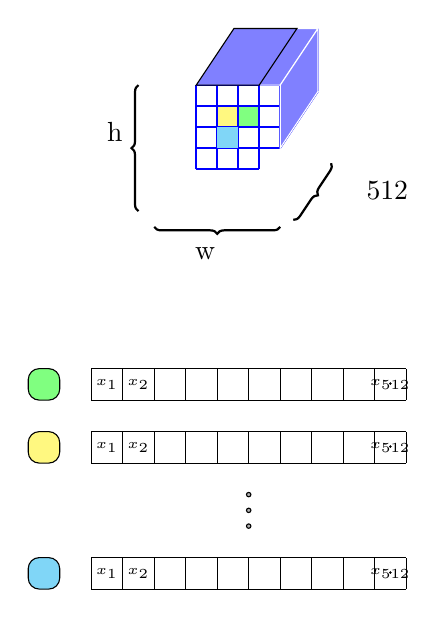
\begin{tikzpicture}[scale=0.8]
	\onslide<1->{
		\renewcommand{\forefillColor}{red!50!white}
		\renewcommand{\borderColor}{white}
		\renewcommand{\toprsidefillcolor}{red!50!white!50}
		\pgfmathsetmacro{\seedx}{0.6}
		\pgfmathsetmacro{\seedy}{1.0}
		\handmadecube{2}{2}{1}{0}{5}

		\draw [
			thick,
			decoration={
				brace,
				mirror,
				raise=0.2cm
			},
			decorate
		] (0,3) -- (0.6,3.9) 
		node [pos=0.1,anchor=north,xshift=-1cm,yshift=-0.4cm] {w}; 

		\draw [
			thick,
			decoration={
				brace,
				mirror,
				raise=0.2cm
			},
			decorate
		] (-2,3) -- (0,3) 
		node [pos=0.1,anchor=north,xshift=2.8cm,yshift=0.5cm] {512};  

		\draw [
			thick,
			decoration={
				brace,
				raise=0.2cm
			},
			decorate
		] (-2,3) -- (-2,5) 
		node [pos=0.1,anchor=north,xshift=-0.5cm,yshift=1.1cm] {h};
		
	}
	
	
	\onslide<3-5>{
		\draw[line width = 0.2mm,step=0.33333,color=blue] (-1,4) grid (0,5);
		\draw [blue,line width = 0.2mm] (-1,4) -- (0,4);
	}
	\onslide<2-5>{
		\fill[green!50!white] (-0.666,4.333) rectangle (-0.333,4.666);

	}
	
	\onslide<5->{
		
		\filldraw[fill=green!50!white, draw=black,rounded corners] (-4,0) rectangle (-3.5,0.5);
		\draw [draw=black,step=0.5] (-3,0) grid (2,0.5);
		\node (x1) at (-2.75,0.25) {\tiny{$x_1$}};
		\node (x2) at (-2.25,0.25) {\tiny{$x_2$}};

		\foreach \x in {-1.75,-1.25,-0.75,-0.25,0.25,0.75,1.25}{
			\node (x2) at (1.75,0.25) {\tiny{$\cdot$}};
		}     
		\node (xn) at (1.75,0.25) {\tiny{$x_{512}$}};
	}
	
	\onslide<5>{
		\draw [blue,line width = 0.2mm] (0,4) -- (0.6,4.9);
		\draw [blue,line width = 0.2mm] (0.6,4.9) -- (0.6,5.9);
		\draw [blue,line width = 0.2mm] (0,5) -- (0.6,5.9);

		\draw [blue,line width = 0.2mm] (-1,5) -- (-0.4,5.9);

		\draw [blue,line width = 0.2mm] (-1,5) -- (-0.4,5.9);

		\draw [blue,line width = 0.2mm] (-0.4,5.9) -- (0.6,5.9);      
		
		\draw  [draw=\borderColor,fill=blue!50] (-1,5) -- (-0.4,5.9) -- (0.6,5.9) -- (0,5)  --cycle ;
		\draw  [draw=\borderColor,fill=blue!50] (0,5)  --(0.6,5.9) -- (0.6,4.9) --(0,4) --cycle ;
	}
	
	
	
	
	\onslide<6>{
		\pgfmathsetmacro\xs{-0.33333};
		\pgfmathsetmacro\ys{0};
		
		\draw[line width = 0.2mm,step=0.33333,color=blue] (-1+\xs,4+\ys) grid (0+\xs,5+\ys);
		\draw [blue,line width = 0.2mm] (-1+\xs,4+\ys) -- (0+\xs,4+\ys);
		
		\draw  [draw=black,fill=blue!50] (-1+\xs,5+\ys) -- (-0.4+\xs,5.9+\ys) -- (0.6+\xs,5.9+\ys) -- (0+\xs,5+\ys)  --cycle ;
		
		%\filldraw[fill=yellow!50!white, draw=black,rounded corners] (-4,0) rectangle (-3.5,0.5);
		
		\fill[yellow!50!white] (-0.666+\xs,4.333+\ys) rectangle (-0.333+\xs,4.666+\ys);
		
	}
	
	\onslide<6->{
		\pgfmathsetmacro\ys{-1cm};
		\filldraw[fill=yellow!50!white, draw=black,rounded corners,yshift=\ys] (-4,0) rectangle (-3.5,0.5);
		\draw [draw=black,step=0.5,yshift=\ys] (-3,0) grid (2,0.5);
		\node[yshift=-0.8cm] (x1) at (-2.75,0.25) {\tiny{$x_1$}};
		\node[yshift=-0.8cm] (x2) at (-2.25,0.25) {\tiny{$x_2$}};

		\foreach \x in {-1.75,-1.25,-0.75,-0.25,0.25,0.75,1.25}{
			\node[yshift=-0.8cm] (x2) at (1.75,0.25) {\tiny{$\cdot$}};
		}     
		\node[yshift=-0.8cm] (xn) at (1.75,0.25) {\tiny{$x_{512}$}};
	}
	
	
	\onslide<7->{
		\filldraw[fill=gray!60!white](-0.5,-1.5)circle(1pt);
		\filldraw[fill=gray!60!white](-0.5,-1.75)circle(1pt);
		\filldraw[fill=gray!60!white](-0.5,-2)circle(1pt);

		\pgfmathsetmacro\ys{-3cm};
		\filldraw[fill=cyan!50!white, draw=black,rounded corners,yshift=\ys] (-4,0) rectangle (-3.5,0.5);
		\draw [draw=black,step=0.5,yshift=\ys] (-3,0) grid (2,0.5);
		\node[yshift=-2.4cm] (x1) at (-2.75,0.25) {\tiny{$x_1$}};
		\node[yshift=-2.4cm] (x2) at (-2.25,0.25) {\tiny{$x_2$}};

		\foreach \x in {-1.75,-1.25,-0.75,-0.25,0.25,0.75,1.25}{
			\node[yshift=-2.4cm] (x2) at (1.75,0.25) {\tiny{$\cdot$}};
		}     
		\node[yshift=-2.4cm] (xn) at (1.75,0.25) {\tiny{$x_{512}$}};
	}
	
	
	\onslide<7>{
		\pgfmathsetmacro\xs{-0.33333};
		\pgfmathsetmacro\ys{-0.33333};
		
		\draw[line width = 0.2mm,step=0.33333,color=blue] (-1+\xs,4+\ys) grid (0+\xs,5+\ys);
		\draw [blue,line width = 0.2mm] (-1+\xs,4+\ys) -- (0+\xs,4+\ys);
		
		%\draw  [draw=black,fill=blue!50] (-1+\xs,5+\ys) -- (-0.4+\xs,5.9+\ys) -- (0.6+\xs,5.9+\ys) -- (0+\xs,5+\ys)  --cycle ;
		
		%\filldraw[fill=cyan!50!white, draw=black,rounded corners] (-4,0) rectangle (-3.5,0.5);
		
		\fill[cyan!50!white] (-0.666+\xs,4.333+\ys) rectangle (-0.333+\xs,4.666+\ys);
		
	}	
\end{tikzpicture}
			\column{0.5\textwidth}
			
			%\begin{footnotesize}
			\begin{itemize}
				\justifying
				\onslide<1->{\item Consider the output of the last convolutional layer of VGGNet }
				\onslide<2->{\item Now consider one cell in one of the $512$ feature maps }
				\onslide<3->{\item If we apply a $3 \times 3$ kernel around this cell then we will get a 1D representation for this cell}
				\onslide<5->{\item If we repeat this for all the $512$ feature maps then we will get a $512$ dimensional representation for this position}
				\onslide<6->{\item We use this process to get a $512$ dimensional representation for each of the $w \times h$ positions}
			\end{itemize}
			
			%\end{footnotesize}
		\end{columns}
		
	\end{overlayarea}
\end{frame}

%%%%%%%%%%%%%%%%%%%%%%%%%%%%%%%%%%%%%%%%%%%%%%%%%%%%%%%%%%%%%%%%%%%%%%%%%%%%%%%%%%%%%%%%%

\begin{frame}
	\begin{overlayarea}{\textwidth}{\textheight}
		\begin{columns}
			\column{0.25\textwidth}
			\begin{tikzpicture}[scale=0.36,rotate=90]
	
	\onslide<1->{
		\renewcommand{\forefillColor}{black!50!white}
		\renewcommand{\borderColor}{white}
		\renewcommand{\toprsidefillcolor}{red}
		\node(image)[scale=0.85,rotate=0] at (-4,-1.5){
			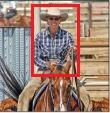
\includegraphics[scale=0.6]{images/cowboy_true.jpg}
		};
		\node[scale=0.85] at (-4,0-5.8){\tiny{Input}};
		
		\draw[->,line width=0.25mm](-2,-1.5)--(0,-1.5);

		\if 0	
		%% input layer
		\handmadecube{0}{4.5}{2.5}{-1}{0}
		\renewcommand{\toprsidefillcolor}{green}                  
		\handmadecube{0}{4.5}{2.5}{-1+0.2}{0}
		\renewcommand{\toprsidefillcolor}{blue!60!white}          
		\handmadecube{0}{4.5}{2.5}{-1+0.4}{0}
		\node[scale=0.85] at (1-0.6*2.6-0.1,0-4.8-0.5){\tiny{Input}};
		%     \node [scale=0.7, rotate=45] at (1-0.6*2.6+0.6,0.2) {\tiny{224}};
		%     \node [scale=0.7, rotate=90] at (1-0.6*2.6+0.2,-2) {\tiny{224}};
		\fi

		% Convolution Layer
		\renewcommand{\forefillColor}{red!50!white}
		\renewcommand{\borderColor}{white}
		\renewcommand{\toprsidefillcolor}{red!50!white!50}

		\pgfmathsetmacro{\seedx}{1}
		\pgfmathsetmacro{\seedy}{0}

		\foreach \xct/\yct in {1,...,2}
		{
			\pgfmathsetmacro{\xcti}{\seedx+\xct*0.1}
			\pgfmathsetmacro{\ycti}{\seedy}
			\handmadecube{0.5}{4.5}{2.5}{\xcti}{\ycti}
		}
		\node[scale=0.85] at (1+0.5,0-4.8){\tiny{Conv}};
		%     \node [scale=0.7, rotate=45] at (1-0.6*2.6+3.2,0.2) {\tiny{224}};
		%     \node [scale=0.7, rotate=90] at (1-0.6*2.6+0.2+2.6,-2) {\tiny{224}};
		%     \node[scale=0.7] at (1+0.725,0-4.2){\tiny{64}};
		
		
		
		% Pooling Layer
		\renewcommand{\forefillColor}{blue!50!white}
		\renewcommand{\borderColor}{white}
		\renewcommand{\toprsidefillcolor}{blue!50!white!50}
		
		\pgfmathsetmacro{\seedx}{2.5}
		\pgfmathsetmacro{\seedy}{0}

		\foreach \xct/\yct in {1}
		{
			%       \pgfmathsetmacro{\xcti}{\seedx+\xct*0.1}
			%       \pgfmathsetmacro{\ycti}{\seedy}
			
			\pgfmathsetmacro{\xcti}{\seedx+\xct*0.1}
			\pgfmathsetmacro{\ycti}{\seedy}
			\handmadecube{0.5}{3.8}{1.8}{\xcti}{\ycti}
		}
		\node[scale=0.85] at (0.5+2.8,0-4.2){\tiny{Max-pool}};
		%     \node [scale=0.6, rotate=45] at (1+3.7,0.2) {\tiny{112}};
		%     \node [scale=0.6, rotate=90] at (1+3.3,-2+0.5) {\tiny{112}};
		%     \node[scale=0.7] at (1+2.85,0-3.5){\tiny{64}};
		
		\foreach \xct in {1,2,3}
		{
			\filldraw[fill=gray!60](3+\xct,-1) circle(2pt) ;
		}

		\draw [thick,step=1,draw=blue!40!white](7,-3) rectangle (11,1);
		\draw [thin,step=0.5,draw=red!40!white](9.5,-0.5) grid (11,1);
		\draw [thin,step=0.5,draw=red!40!white](9.5,-0.5) -- (9.5,1);

		\filldraw[fill=green!50!white, draw=black,rounded corners] (13,4) rectangle (14,5);
		\draw [thin,step=1,draw=blue!40!white](7,-3) rectangle (11,1);
		\draw (13,-5) grid[xstep=1,ystep=1] (14,3);
		\node (x1) at (13.5,2.5) {\tiny{$x_1$}};
		\node (x2) at (13.5,1.5) {\tiny{$x_2$}};

		\foreach \y in {1,2,...,5}{
			\node (x2) at (13.5,1.5-\y) {\tiny{$\cdot$}};
		}

		\node (x2) at (13.5,-4.5) {\tiny{$x_{512}$}};
				
		\draw[->](11.1,-1)--(12.8,-1);
	}
	
	
	
\end{tikzpicture}		
			\column{0.25\textwidth}
			\begin{tikzpicture}
	\hspace*{0.5cm}
	\onslide<2->{
		
		\node(image)[scale=0.55,rotate=0] at (0,0){
			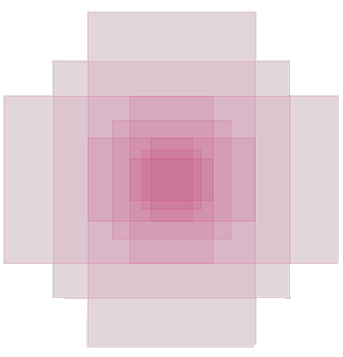
\includegraphics[scale=0.6]{images/achor_boxes_crop.png}
		};
		
	}
	
\end{tikzpicture}
			\column{0.5\textwidth}
			\begin{itemize}
				\justifying
				\onslide<2->{\item We now consider $k$ bounding boxes (called anchor boxes) of different sizes \& aspect ratio}
				\onslide<3->{\item We are interested in the following two questions: }
				\onslide<4->{\item Given the $512d$ representation of a position, what is the probability that a given anchor box centered at this position contains an object?}
				
				\onslide<5->{
					(Classification)
				}
				\onslide<6->{\item How do you predict the true bounding box from this anchor box?}
				\onslide<7->{
					(Regression)
				}
				%\onslide<5->{\item }
				%\onslide<6->{\item }
			\end{itemize}
		\end{columns}
	\end{overlayarea}
\end{frame}

%%%%%%%%%%%%%%%%%%%%%%%%%%%%%%%%%%%%%%%%%%%%%%%%%%%%%%%%%%%%%%%%%%%%%%%%%%%%%%%%%%%%%%%%%			

\begin{frame}
	\begin{overlayarea}{\textwidth}{\textheight}
		\begin{columns}

			\column{0.3\textwidth}
			\begin{tikzpicture}[scale=0.36,rotate=90]
	
	\onslide<1->{
		\renewcommand{\forefillColor}{black!50!white}
		\renewcommand{\borderColor}{white}
		\renewcommand{\toprsidefillcolor}{red}
		\node(image)[scale=0.85,rotate=0] at (-4,-1.5){
			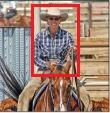
\includegraphics[scale=0.6]{images/cowboy_true.jpg}
		};
		\node[scale=0.85] at (-4,0-5.8){\tiny{Input}};
		
		\draw[->,line width=0.25mm](-2,-1.5)--(0,-1.5);

		\if 0
		%% input layer
		\handmadecube{0}{4.5}{2.5}{-1}{0}
		\renewcommand{\toprsidefillcolor}{green}                  
		\handmadecube{0}{4.5}{2.5}{-1+0.2}{0}
		\renewcommand{\toprsidefillcolor}{blue!60!white}          
		\handmadecube{0}{4.5}{2.5}{-1+0.4}{0}
		\node[scale=0.85] at (1-0.6*2.6-0.1,0-4.8-0.5){\tiny{Input}};
		%     \node [scale=0.7, rotate=45] at (1-0.6*2.6+0.6,0.2) {\tiny{224}};
		%     \node [scale=0.7, rotate=90] at (1-0.6*2.6+0.2,-2) {\tiny{224}};
		\fi

		% Convolution Layer
		\renewcommand{\forefillColor}{red!50!white}
		\renewcommand{\borderColor}{white}
		\renewcommand{\toprsidefillcolor}{red!50!white!50}
		
		\pgfmathsetmacro{\seedx}{1}
		\pgfmathsetmacro{\seedy}{0}

		\foreach \xct/\yct in {1,...,2}
		{
			\pgfmathsetmacro{\xcti}{\seedx+\xct*0.1}
			\pgfmathsetmacro{\ycti}{\seedy}
			\handmadecube{0.5}{4.5}{2.5}{\xcti}{\ycti}
		}
		\node[scale=0.85] at (1+0.5,0-4.8){\tiny{Conv}};
		%     \node [scale=0.7, rotate=45] at (1-0.6*2.6+3.2,0.2) {\tiny{224}};
		%     \node [scale=0.7, rotate=90] at (1-0.6*2.6+0.2+2.6,-2) {\tiny{224}};
		%     \node[scale=0.7] at (1+0.725,0-4.2){\tiny{64}};
		
		
		
		% Pooling Layer
		\renewcommand{\forefillColor}{blue!50!white}
		\renewcommand{\borderColor}{white}
		\renewcommand{\toprsidefillcolor}{blue!50!white!50}
		
		\pgfmathsetmacro{\seedx}{2.5}
		\pgfmathsetmacro{\seedy}{0}

		\foreach \xct/\yct in {1}
		{
			%       \pgfmathsetmacro{\xcti}{\seedx+\xct*0.1}
			%       \pgfmathsetmacro{\ycti}{\seedy}
			
			\pgfmathsetmacro{\xcti}{\seedx+\xct*0.1}
			\pgfmathsetmacro{\ycti}{\seedy}
			\handmadecube{0.5}{3.8}{1.8}{\xcti}{\ycti}
		}
		\node[scale=0.85] at (0.5+2.8,0-4.2){\tiny{Max-pool}};
		%     \node [scale=0.6, rotate=45] at (1+3.7,0.2) {\tiny{112}};
		%     \node [scale=0.6, rotate=90] at (1+3.3,-2+0.5) {\tiny{112}};
		%     \node[scale=0.7] at (1+2.85,0-3.5){\tiny{64}};
		
		\foreach \xct in {1,2,3}
		{
			\filldraw[fill=gray!60](3+\xct,-1) circle(2pt) ;
		}

		\draw [thick,step=1,draw=blue!40!white](7,-3) rectangle (11,1);
		\draw [thin,step=0.5,draw=red!40!white](9.5,-0.5) grid (11,1);
		\draw [thin,step=0.5,draw=red!40!white](9.5,-0.5) -- (9.5,1);

		\filldraw[fill=green!50!white, draw=black,rounded corners] (13,4) rectangle (14,5);
		\draw [thin,step=1,draw=blue!40!white](7,-3) rectangle (11,1);
		\draw (13,-5) grid[xstep=1,ystep=1] (14,3);     
		\node (x1) at (13.5,2.5) {\tiny{$x_1$}};
		\node (x2) at (13.5,1.5) {\tiny{$x_2$}};

		\foreach \y in {1,2,...,5}{
			\node (x2) at (13.5,1.5-\y) {\tiny{$\cdot$}};
		}

		\node (x2) at (13.5,-4.5) {\tiny{$x_{512}$}};

		\draw[->](11.1,-1)--(12.8,-1);
	}
	
	
	
\end{tikzpicture}
			
			\column{0.25\textwidth}
			\begin{tikzpicture}
	\hspace*{0.5cm}
	%\onslide<2->{
		
		\node(image)[scale=0.55,rotate=0] at (0,0){
			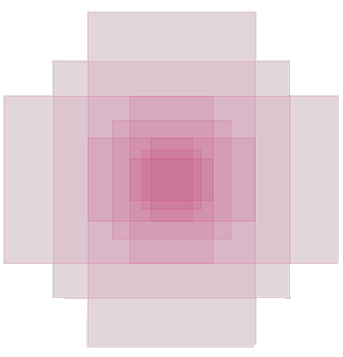
\includegraphics[scale=0.6]{images/achor_boxes_crop.png}
		};
		
	%}
	
\end{tikzpicture}
			\column{0.5\textwidth}

			\begin{itemize}
				\justifying
				\onslide<1->{\item We train a classification model and a regression model to address these two questions}
				\onslide<2->{\item \textcolor<4->{red}{How do we get the ground truth data?}}
				\onslide<3->{\item What is the objective function used for training?}
			\end{itemize}

		\end{columns}
	\end{overlayarea}     
\end{frame}

%%%%%%%%%%%%%%%%%%%%%%%%%%%%%%%%%%%%%%%%%%%%%%%%%%%%%%%%%%%%%%%%%%%%%%%%%%%%%%%%%%%%%%%%%

\begin{frame}
	\begin{overlayarea}{\textwidth}{\textheight}
		\begin{columns}

			\column{0.3\textwidth}
						\begin{tikzpicture}	[scale=0.25,rotate=90]	
			\centering
			\onslide<1->{
				\node(image)[scale=0.85,rotate=0] at (-5,-1.5){
					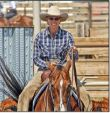
\includegraphics[scale=0.6]{images/cowboy.JPG}
				};

				\node[scale=0.85] at (-5,0-5.8){\tiny{Input}};
			}
				
			\onslide<2->{
					\renewcommand{\forefillColor}{black!50!white}
					\renewcommand{\borderColor}{white}
					\renewcommand{\toprsidefillcolor}{red}
				\node(image)[scale=0.85,rotate=0] at (-5,-1.5){
										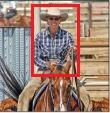
\includegraphics[scale=0.6]{images/cowboy_true.jpg}
									};
					\draw[->,line width=0.25mm](-2,-1.5)--(0,-1.5);
						% Convolution Layer
						\renewcommand{\forefillColor}{red!50!white}
						\renewcommand{\borderColor}{white}
						\renewcommand{\toprsidefillcolor}{red!50!white!50}
						\pgfmathsetmacro{\seedx}{1}
						\pgfmathsetmacro{\seedy}{0}
										
						\foreach \xct/\yct in {1,...,2}
						{
							\pgfmathsetmacro{\xcti}{\seedx+\xct*0.1}
							\pgfmathsetmacro{\ycti}{\seedy}
							\handmadecube{0.5}{4.5}{2.5}{\xcti}{\ycti}
						}
						\node[scale=0.85] at (1+0.5,0-4.8){\tiny{Conv}};
					
									% Pooling Layer
									\renewcommand{\forefillColor}{blue!50!white}
									\renewcommand{\borderColor}{white}
									\renewcommand{\toprsidefillcolor}{blue!50!white!50}
									
									\pgfmathsetmacro{\seedx}{2.5}
									\pgfmathsetmacro{\seedy}{0}
									
									\foreach \xct/\yct in {1}
									{
										%				\pgfmathsetmacro{\xcti}{\seedx+\xct*0.1}
										%				\pgfmathsetmacro{\ycti}{\seedy}
										
										\pgfmathsetmacro{\xcti}{\seedx+\xct*0.1}
										\pgfmathsetmacro{\ycti}{\seedy}
										\handmadecube{0.5}{3.8}{1.8}{\xcti}{\ycti}
									}
									\node[scale=0.85] at (0.5+2.8,0-4.2){\tiny{Max-pool}};
					}
			\onslide<3->{
											
				\foreach \xct in {1,2,3}
				{
					\filldraw[fill=gray!60](3+\xct,-1) circle(2pt) ;
				}
							
				\draw [thin,step=0.7,draw=blue!40!white](6.4,-4.2) grid (12.5,1.4);			
				%\draw [draw=blue!40,thin](6.4,-4.3) grid[step=0.5] (12.5,1.5);
				%\draw [draw=blue!40,thin] (6.4,-4.3) -- (12.5,-4.3);
				\draw [draw=blue!40,thin] (6.4,-4.2) -- (6.4,1.4);
				\draw [draw=blue!40,thin] (12.5,-4.2) -- (12.5,1.4);
			}
		
		\if 0	
		\onslide<4->{			
						
			\pgfmathsetmacro{\x}{10-1}
			\pgfmathsetmacro{\y}{0-1}
						
						\pgfmathsetmacro{\x}{\x-0.5}
						\pgfmathsetmacro{\y}{\y-1.8}
						%\filldraw[fill=red, draw=red,line width=0.5mm] (\x+1.4,\y+0.85) rectangle (\x+1.9,\y+1.35);
						\draw[draw=red,line width=0.4mm] (\x,\y) rectangle (\x+3.5,\y+2.5);		
					}
		\fi		
			\onslide<3->{			
				\pgfmathsetmacro{\x}{10-1}
				\pgfmathsetmacro{\y}{0-1}
									
				\pgfmathsetmacro{\x}{\x-0.5}
				\pgfmathsetmacro{\y}{\y-1.8}
				\filldraw[fill=green, draw=green,line width=0.5mm] (\x+0.7,\y+0.75) rectangle (\x+1.2,\y+1.25);			
			
			%\draw[draw=green,line width=0.7mm] (\x-0.5,\y-0.5) rectangle (\x+2.5,\y+2.5);			
			
			%\node (A1) at (9.5,-3) {};			
			%\node (A3) at (13,-16.1) {};	
			%\path [->,line width=0.3mm] (A3) edge (A1);
							
		}
		\onslide<4->{
			\node(image)[scale=0.85,rotate=0] at (-5,-1.5){
				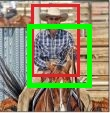
\includegraphics[scale=0.6]{images/cowboy_true_green.jpg}
			};

			\node[scale=0.85] at (-5,0-5.8){\tiny{Input}};
		}
	    \onslide<5->{
   			\node(image)[scale=0.85,rotate=0] at (-5,-1.5){
   				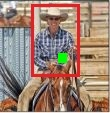
\includegraphics[scale=0.6]{images/cowboy_true_centre.jpg}
   			};
	    
   			\node[scale=0.85] at (-5,0-5.8){\tiny{Input}};
   		}
   		\onslide<7->{
			\colorlet{custom_pink}{pink!50}
			
			\newcommand{\lightercolor}[3]{% Reference Color, Percentage, New Color Name
	    	\colorlet{#3}{#1!#2!white}
			}
			\lightercolor{custom_pink}{30}{LightPink}
	 					
			\filldraw[fill=pink, draw=pink,line width=0.5mm, opacity = 0.7] (-7,-3) rectangle (-3,-1);
  			%\node(image)[scale=0.9,rotate=0] at (-5,-2.2){
  			%	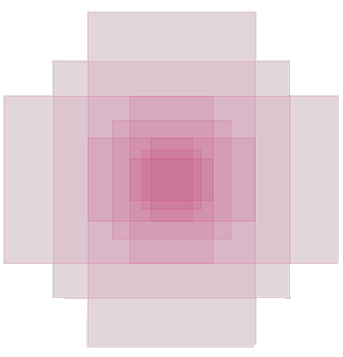
\includegraphics[scale=0.08]{images/achor_boxes_crop.png}
  			%};

  			%\node[scale=0.85] at (-5,0-5.8){\tiny{Input}};
   		}
							
		\onslide<7->{
					\draw (13,-5) grid[xstep=1,ystep=1] (14,3);			
					\node (x1) at (13.5,2.5) {\tiny{$x_1$}};
					\node (x2) at (13.5,1.5) {\tiny{$x_2$}};
					
					\foreach \y in {1,2,...,5}{
						\node (x2) at (13.5,1.5-\y) {\tiny{$\cdot$}};
					}
					
					\node (x2) at (13.5,-4.5) {\tiny{$\cdot$}};
					
					\draw[->](11.8,-1)--(12.8,-1);
					
					\node(A) at (13.5,-1){};
					\node(B)[draw,rounded corners] at (16.5,3){\scriptsize{Classification}};
					\path[draw,line width=0.25mm,->] (A) edge (B);		
					
		}
		\onslide<8->{
			\node(C)[draw,rounded corners] at (16.5,-5){\scriptsize{Regression}};
			\path[draw,line width=0.25mm,->] (A) edge (C);
		}
							
			
			\end{tikzpicture}
			
			\column{0.2\textwidth}
			\begin{tikzpicture}[scale=1]
			\onslide<6->{
						\node(image)[scale=0.55,rotate=0] at (0,0){
										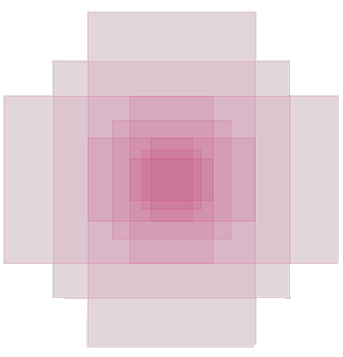
\includegraphics[scale=0.6]{images/achor_boxes_crop.png}
									};
					}
			\end{tikzpicture}
			\if 0
			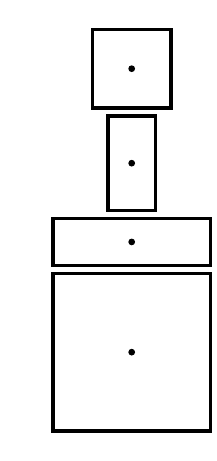
\begin{tikzpicture}[scale=1]
			\hspace*{0.3cm}
			\onslide<3->{
				
				\draw[black, very thick] (0,0)rectangle (2,2);
				\draw[black, very thick] (0,2.1)rectangle (2,2.7);
				\draw[black, very thick] (0.7,2.8)rectangle (1.3,4);
				\draw[black, very thick] (0.5,4.1)rectangle (1.5,5.1);
				
				\filldraw [black] (1,1) circle (1pt);
				\filldraw [black] (1,2.4) circle (1pt);
				\filldraw [black] (1,3.4) circle (1pt);
				\filldraw [black] (1,4.6) circle (1pt);
				
			}
			
			\end{tikzpicture}
			\fi

			\column{0.5\textwidth}

			\begin{itemize}
				\justifying
				\only<1-6>{
				\item<1-> Consider a ground truth object and its corresponding bounding box 
				\item<2-> Consider the projection of this image onto the conv5 layer
				%\item<3-> For every cell in the output, we place an anchor box at the center of the region which corresponds to this cell
				\item<3-> Consider one such cell in the output
				\item<4-> This cell corresponds to a patch in the original image
				\item<5-> Consider the center of this patch
				\item<6-> We consider anchor boxes of different sizes
				}
				\only<7-8>{
				\item<7-> For each of these anchor boxes, we would want the classifier to predict 1 if this anchor box has a reasonable overlap (IoU $>$ 0.7) with the true grounding box
				\item<8-> Similarly we would want the regression model to predict the true box (red) from the anchor box (pink) 
				}
			\end{itemize}

		\end{columns}
	\end{overlayarea}     
\end{frame}
			
%%%%%%%%%%%%%%%%%%%%%%%%%%%%%%%%%%%%%%%%%%%%%%%%%%%%%%%%%%%%%%%%%%%%%%%%%%%%%%%%%%%%%%%%%

\begin{frame}
	\begin{overlayarea}{\textwidth}{\textheight}
		\begin{columns}

			\column{0.3\textwidth}
							\begin{tikzpicture}	[scale=0.25,rotate=90]	
			\centering
			\onslide<1->{
				\node(image)[scale=0.85,rotate=0] at (-5,-1.5){
					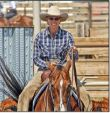
\includegraphics[scale=0.6]{images/cowboy.JPG}
				};

				\node[scale=0.85] at (-5,0-5.8){\tiny{Input}};
			}
				
			\onslide<1->{
					\renewcommand{\forefillColor}{black!50!white}
					\renewcommand{\borderColor}{white}
					\renewcommand{\toprsidefillcolor}{red}
				\node(image)[scale=0.85,rotate=0] at (-5,-1.5){
										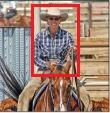
\includegraphics[scale=0.6]{images/cowboy_true.jpg}
									};
					\draw[->,line width=0.25mm](-2,-1.5)--(0,-1.5);
						% Convolution Layer
						\renewcommand{\forefillColor}{red!50!white}
						\renewcommand{\borderColor}{white}
						\renewcommand{\toprsidefillcolor}{red!50!white!50}
						\pgfmathsetmacro{\seedx}{1}
						\pgfmathsetmacro{\seedy}{0}
										
						\foreach \xct/\yct in {1,...,2}
						{
							\pgfmathsetmacro{\xcti}{\seedx+\xct*0.1}
							\pgfmathsetmacro{\ycti}{\seedy}
							\handmadecube{0.5}{4.5}{2.5}{\xcti}{\ycti}
						}
						\node[scale=0.85] at (1+0.5,0-4.8){\tiny{Conv}};
					
									% Pooling Layer
									\renewcommand{\forefillColor}{blue!50!white}
									\renewcommand{\borderColor}{white}
									\renewcommand{\toprsidefillcolor}{blue!50!white!50}
									
									\pgfmathsetmacro{\seedx}{2.5}
									\pgfmathsetmacro{\seedy}{0}
									
									\foreach \xct/\yct in {1}
									{
										%				\pgfmathsetmacro{\xcti}{\seedx+\xct*0.1}
										%				\pgfmathsetmacro{\ycti}{\seedy}
										
										\pgfmathsetmacro{\xcti}{\seedx+\xct*0.1}
										\pgfmathsetmacro{\ycti}{\seedy}
										\handmadecube{0.5}{3.8}{1.8}{\xcti}{\ycti}
									}
									\node[scale=0.85] at (0.5+2.8,0-4.2){\tiny{Max-pool}};
					}
			\onslide<1->{
											
				\foreach \xct in {1,2,3}
				{
					\filldraw[fill=gray!60](3+\xct,-1) circle(2pt) ;
				}
							
				\draw [thin,step=0.7,draw=blue!40!white](6.4,-4.2) grid (12.5,1.4);			
				%\draw [draw=blue!40,thin](6.4,-4.3) grid[step=0.5] (12.5,1.5);
				%\draw [draw=blue!40,thin] (6.4,-4.3) -- (12.5,-4.3);
				\draw [draw=blue!40,thin] (6.4,-4.2) -- (6.4,1.4);
				\draw [draw=blue!40,thin] (12.5,-4.2) -- (12.5,1.4);
			}
		
			\onslide<1->{			
				\pgfmathsetmacro{\x}{10-1}
				\pgfmathsetmacro{\y}{0-1}
									
				\pgfmathsetmacro{\x}{\x-0.5}
				\pgfmathsetmacro{\y}{\y-1.8}
				%\filldraw[fill=green, draw=green,line width=0.5mm] (\x+0.7,\y+0.75) rectangle (\x+1.2,\y+1.25);			
			
			%\draw[draw=green,line width=0.7mm] (\x-0.5,\y-0.5) rectangle (\x+2.5,\y+2.5);			
			
			%\node (A1) at (9.5,-3) {};			
			%\node (A3) at (13,-16.1) {};	
			%\path [->,line width=0.3mm] (A3) edge (A1);
							
		}
							
		\onslide<1->{
					\draw (13,-5) grid[xstep=1,ystep=1] (14,3);			
					\node (x1) at (13.5,2.5) {\tiny{$x_1$}};
					\node (x2) at (13.5,1.5) {\tiny{$x_2$}};
					
					\foreach \y in {1,2,...,5}{
						\node (x2) at (13.5,1.5-\y) {\tiny{$\cdot$}};
					}
					
					\node (x2) at (13.5,-4.5) {\tiny{$\cdot$}};
					
					\draw[->](11.8,-1)--(12.8,-1);
					
					\node(A) at (13.5,-1){};
					\node(B)[draw,rounded corners] at (16.5,3){\scriptsize{Classification}};
					\path[draw,line width=0.25mm,->] (A) edge (B);		
					
		}
		\onslide<1->{
			\node(C)[draw,rounded corners] at (16.5,-5){\scriptsize{Regression}};
			\path[draw,line width=0.25mm,->] (A) edge (C);
		}
							
			
			\end{tikzpicture}
			
			\column{0.2\textwidth}
			\begin{tikzpicture}[scale=1]
			\onslide<1->{
						\node(image)[scale=0.55,rotate=0] at (0,0){
										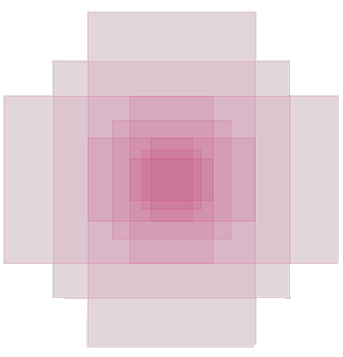
\includegraphics[scale=0.6]{images/achor_boxes_crop.png}
									};
					}
			\end{tikzpicture}

			
			%\column{0.25\textwidth}
			%	\begin{tikzpicture}
	\hspace*{0.5cm}
	%\onslide<2->{
		
		\node(image)[scale=0.55,rotate=0] at (0,0){
			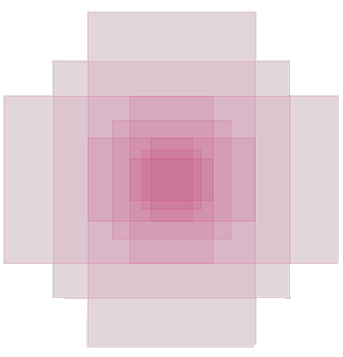
\includegraphics[scale=0.6]{images/achor_boxes_crop.png}
		};
		
	%}
	
\end{tikzpicture}
			\column{0.5\textwidth}

			\begin{itemize}
				\justifying
				\item We train a classification model and a regression model to address these two questions
				\item How do we get the ground truth data?
				\item \textcolor<1->{red}{What is the objective function used for training?}
			\end{itemize}

		\end{columns}
	\end{overlayarea}     
\end{frame}

	
%%%%%%%%%%%%%%%%%%%%%%%%%%%%%%%%%%%%%%%%%%%%%%%%%%%%%%%%%%%%%%%%%%%%%%%%%%%%%%%%%%%%%%%%%

\begin{frame}
	\begin{itemize}
		\item The full network is trained using the following objective.
	\end{itemize}
	\begin{equation*}
		\onslide<2-> {\mathscr{L}({p_i}, {t_i}) = \frac{1}{N_{cls}} \sum_{i} \mathscr{L}_{cls}(p_i,p_{i}^*)} \onslide<4->{+ \frac{\lambda}{N_{reg}} \sum_{i} p_i^* \mathscr{L}_{reg}(t_i,t_i^*)}
	\end{equation*}
	
	\begin{align*}
		\onslide<3->{
			p_i^* & = 1 \text{\quad if anchor box contains ground truth object}        \\
	& = 0 \text{\quad otherwise}                                          \\
			p_i   & = \text{predicted probability of anchor box containing an object } \\ 
			N_{cls}& = \text{batch-size}
		}    
		\onslide<5->{                                            \\
			N_{reg}&= \text{batch-size} \times k						\\
			k     & = \text{anchor boxes}
		}                                               
	\end{align*}
\end{frame}

%%%%%%%%%%%%%%%%%%%%%%%%%%%%%%%%%%%%%%%%%%%%%%%%%%%%%%%%%%%%%%%%%%%%%%%%%%%%%%%%%%%%%%%%%		
			
\begin{frame}
	\begin{columns}
		\column{0.5\textwidth}
			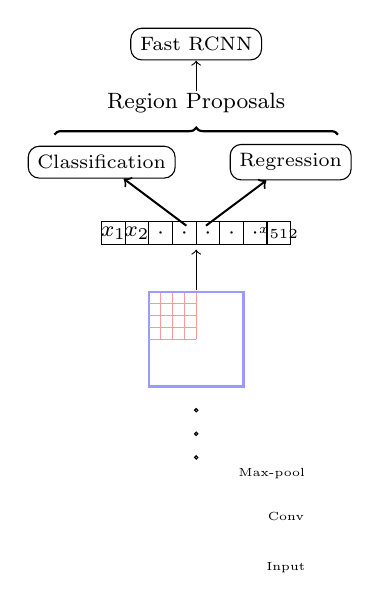
\begin{tikzpicture} [scale=0.30,rotate=90]  
	%\onslide<1>{\draw[draw=red!50,fill=red!10,thick,solid,rounded corners] (-2,-6) rectangle (11.5,3); }
	%\onslide<2>{\draw[draw=red!50,fill=red!10,thick,solid,rounded corners] (15,-8.5) rectangle (19.5,6); }
	%\onslide<3>{\draw[draw=red!50,fill=red!10,thick,solid,rounded corners] (20,-5) rectangle (24,3); }
	
	\onslide<1->{

		\renewcommand{\forefillColor}{black!50!white}
		\renewcommand{\borderColor}{white}
		\renewcommand{\toprsidefillcolor}{red}

		%% input layer
		\handmadecube{0}{4.5}{2.5}{-1}{0}
		\renewcommand{\toprsidefillcolor}{green}                  
		\handmadecube{0}{4.5}{2.5}{-1+0.2}{0}
		\renewcommand{\toprsidefillcolor}{blue!60!white}          
		\handmadecube{0}{4.5}{2.5}{-1+0.4}{0}
		\node[scale=0.85] at (1-0.6*2.6-0.1,0-4.8){\tiny{Input}};
		%     \node [scale=0.7, rotate=45] at (1-0.6*2.6+0.6,0.2) {\tiny{224}};
		%     \node [scale=0.7, rotate=90] at (1-0.6*2.6+0.2,-2) {\tiny{224}};


		% Convolution Layer
		\renewcommand{\forefillColor}{red!50!white}
		\renewcommand{\borderColor}{white}
		\renewcommand{\toprsidefillcolor}{red!50!white!50}

		\pgfmathsetmacro{\seedx}{1}
		\pgfmathsetmacro{\seedy}{0}

		\foreach \xct/\yct in {1,...,2}
		{
			\pgfmathsetmacro{\xcti}{\seedx+\xct*0.1}
			\pgfmathsetmacro{\ycti}{\seedy}
			\handmadecube{0.5}{4.5}{2.5}{\xcti}{\ycti}
		}
		\node[scale=0.85] at (1+0.5,0-4.8){\tiny{Conv}};
		%     \node [scale=0.7, rotate=45] at (1-0.6*2.6+3.2,0.2) {\tiny{224}};
		%     \node [scale=0.7, rotate=90] at (1-0.6*2.6+0.2+2.6,-2) {\tiny{224}};
		%     \node[scale=0.7] at (1+0.725,0-4.2){\tiny{64}};
		
		
		
		% Pooling Layer
		\renewcommand{\forefillColor}{blue!50!white}
		\renewcommand{\borderColor}{white}
		\renewcommand{\toprsidefillcolor}{blue!50!white!50}
		
		\pgfmathsetmacro{\seedx}{2.5}
		\pgfmathsetmacro{\seedy}{0}

		\foreach \xct/\yct in {1}
		{
			%       \pgfmathsetmacro{\xcti}{\seedx+\xct*0.1}
			%       \pgfmathsetmacro{\ycti}{\seedy}
			
			\pgfmathsetmacro{\xcti}{\seedx+\xct*0.1}
			\pgfmathsetmacro{\ycti}{\seedy}
			\handmadecube{0.5}{3.8}{1.8}{\xcti}{\ycti}
		}
		\node[scale=0.85] at (0.5+2.8,0-4.2){\tiny{Max-pool}};
		%     \node [scale=0.6, rotate=45] at (1+3.7,0.2) {\tiny{112}};
		%     \node [scale=0.6, rotate=90] at (1+3.3,-2+0.5) {\tiny{112}};
		%     \node[scale=0.7] at (1+2.85,0-3.5){\tiny{64}};
		
		\foreach \xct in {1,2,3}
		{
			\filldraw[fill=gray!60](3+\xct,-1) circle(2pt) ;
		}

		\draw [thick,step=1,draw=blue!40!white](7,-3) rectangle (11,1);
		\draw [thin,step=0.5,draw=red!40!white](9,-1) grid (11,1);
		\draw [thin,step=0.5,draw=red!40!white](9,-1) -- (9,1);

		%     \filldraw[fill=green!50!white, draw=black,rounded corners] (13,4) rectangle (14,5);
		\draw [thin,step=1,draw=blue!40!white](7,-3) rectangle (11,1);
		\draw (13,-5) grid[xstep=1,ystep=1] (14, 3);     
		\node (x1) at (13.5,2.5) {\footnotesize{$x_1$}};
		\node (x2) at (13.5,1.5) {\footnotesize{$x_2$}};

		\foreach \y in {1,2,...,5}{
			\node (x2) at (13.5,1.5-\y) {\footnotesize{$\cdot$}};
		}

		\node (x2) at (13.5,-4.5) {\tiny{$x_{512}$}};

		\draw[->](11.1,-1)--(12.8,-1);

		\node(A) at (13.5,-1){};
		\node(B)[draw,rounded corners] at (16.5,3){\scriptsize{Classification}};
		\node(C)[draw,rounded corners] at (16.5,-5){\scriptsize{Regression}};
		\node(D)[draw,rounded corners] at (21.5,-1){\scriptsize{Fast RCNN}};
		\path[draw,line width=0.25mm,->] (A) edge (B);
		\path[draw,line width=0.25mm,->] (A) edge (C);
		%\node(D)[draw,rounded corners] at (20.5.5,3){\scriptsize{Classification}};
		\draw[->](19.5,-1)--(20.8,-1);
		\node[font=\fontsize{8}{10}\selectfont] at (19,-1) {Region Proposals};

		\draw [
			thick,
			decoration={
				brace,
				raise=0.2cm
			},
			decorate
		] (17,5) -- (17,-7) 
		node [pos=0.1,anchor=north,xshift=-0.5cm,yshift=1.1cm] {};
		

	}
\end{tikzpicture}

		\column{0.5\textwidth}
		\begin{overlayarea}{\textwidth}{\textheight}
			\begin{itemize}
				\justifying
				\item<2-> So far we have seen a CNN based approach for region proposals instead of using selective search
				\item<3-> We can now take these region proposals and then add fast RCNN on top of it to predict the class of the object
				\item <4-> And regress the proposed bounding box
			\end{itemize}
		\end{overlayarea}
	\end{columns}
\end{frame}
						
%%%%%%%%%%%%%%%%%%%%%%%%%%%%%%%%%%%%%%%%%%%%%%%%%%%%%%%%%%%%%%%%%%%%%%%%%%%%%%%%%%%%%%%%%	

\begin{frame}
	\begin{columns}
		\column{0.5\textwidth}
			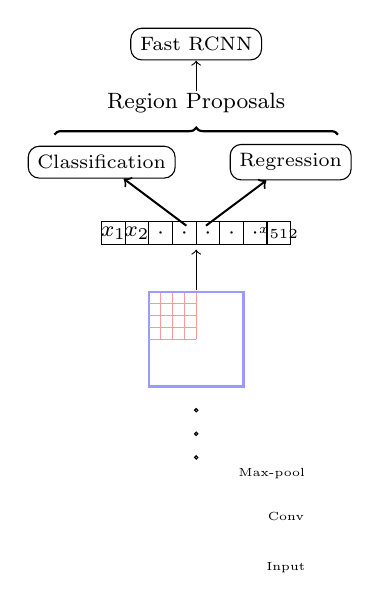
\begin{tikzpicture} [scale=0.30,rotate=90]  
	% \onslide<1>{\draw[draw=red!50,fill=red!10,thick,solid,rounded corners] (-2,-6) rectangle (11.5,3); }
	% \onslide<2>{\draw[draw=red!50,fill=red!10,thick,solid,rounded corners] (15,-8.5) rectangle (19.5,6); }
	%\onslide<3>{\draw[draw=red!50,fill=red!10,thick,solid,rounded corners] (20,-5) rectangle (24,3); }
	
	\onslide<1->{

		\renewcommand{\forefillColor}{black!50!white}
		\renewcommand{\borderColor}{white}
		\renewcommand{\toprsidefillcolor}{red}

		%% input layer
		\handmadecube{0}{4.5}{2.5}{-1}{0}
		\renewcommand{\toprsidefillcolor}{green}                  
		\handmadecube{0}{4.5}{2.5}{-1+0.2}{0}
		\renewcommand{\toprsidefillcolor}{blue!60!white}          
		\handmadecube{0}{4.5}{2.5}{-1+0.4}{0}
		\node[scale=0.85] at (1-0.6*2.6-0.1,0-4.8){\tiny{Input}};
		%     \node [scale=0.7, rotate=45] at (1-0.6*2.6+0.6,0.2) {\tiny{224}};
		%     \node [scale=0.7, rotate=90] at (1-0.6*2.6+0.2,-2) {\tiny{224}};


		% Convolution Layer
		\renewcommand{\forefillColor}{red!50!white}
		\renewcommand{\borderColor}{white}
		\renewcommand{\toprsidefillcolor}{red!50!white!50}

		\pgfmathsetmacro{\seedx}{1}
		\pgfmathsetmacro{\seedy}{0}

		\foreach \xct/\yct in {1,...,2}
		{
			\pgfmathsetmacro{\xcti}{\seedx+\xct*0.1}
			\pgfmathsetmacro{\ycti}{\seedy}
			\handmadecube{0.5}{4.5}{2.5}{\xcti}{\ycti}
		}
		\node[scale=0.85] at (1+0.5,0-4.8){\tiny{Conv}};
		%     \node [scale=0.7, rotate=45] at (1-0.6*2.6+3.2,0.2) {\tiny{224}};
		%     \node [scale=0.7, rotate=90] at (1-0.6*2.6+0.2+2.6,-2) {\tiny{224}};
		
		%     \node[scale=0.7] at (1+0.725,0-4.2){\tiny{64}};
		
		
		
		% Pooling Layer
		\renewcommand{\forefillColor}{blue!50!white}
		\renewcommand{\borderColor}{white}
		\renewcommand{\toprsidefillcolor}{blue!50!white!50}
		
		\pgfmathsetmacro{\seedx}{2.5}
		\pgfmathsetmacro{\seedy}{0}

		\foreach \xct/\yct in {1}
		{
			%       \pgfmathsetmacro{\xcti}{\seedx+\xct*0.1}
			%       \pgfmathsetmacro{\ycti}{\seedy}
			
			\pgfmathsetmacro{\xcti}{\seedx+\xct*0.1}
			\pgfmathsetmacro{\ycti}{\seedy}
			\handmadecube{0.5}{3.8}{1.8}{\xcti}{\ycti}
		}
		\node[scale=0.85] at (0.5+2.8,0-4.2){\tiny{Max-pool}};
		%     \node [scale=0.6, rotate=45] at (1+3.7,0.2) {\tiny{112}};
		%     \node [scale=0.6, rotate=90] at (1+3.3,-2+0.5) {\tiny{112}};
		%     \node[scale=0.7] at (1+2.85,0-3.5){\tiny{64}};
		
		\foreach \xct in {1,2,3}
		{
			\filldraw[fill=gray!60](3+\xct,-1) circle(2pt) ;
		}

		\draw [thick,step=1,draw=blue!40!white](7,-3) rectangle (11,1);
		\draw [thin,step=0.5,draw=red!40!white](9,-1) grid (11,1);
		\draw [thin,step=0.5,draw=red!40!white](9,-1) -- (9,1);

		%     \filldraw[fill=green!50!white, draw=black,rounded corners] (13,4) rectangle (14,5);
		\draw [thin,step=1,draw=blue!40!white](7,-3) rectangle (11,1);
		\draw (13,-5) grid[xstep=1,ystep=1] (14,3);     
		\node (x1) at (13.5,2.5) {\footnotesize{$x_1$}};
		\node (x2) at (13.5,1.5) {\footnotesize{$x_2$}};

		\foreach \y in {1,2,...,5}{
			\node (x2) at (13.5,1.5-\y) {\footnotesize{$\cdot$}};
		}

		\node (x2) at (13.5,-4.5) {\tiny{$x_{512}$}};

		\draw[->](11.1,-1)--(12.8,-1);

		\node(A) at (13.5,-1){};
		\node(B)[draw,rounded corners] at (16.5,3){\scriptsize{Classification}};
		\node(C)[draw,rounded corners] at (16.5,-5){\scriptsize{Regression}};
		\node(D)[draw,rounded corners] at (21.5,-1){\scriptsize{Fast RCNN}};
		\path[draw,line width=0.25mm,->] (A) edge (B);
		\path[draw,line width=0.25mm,->] (A) edge (C);
		%\node(D)[draw,rounded corners] at (20.5.5,3){\scriptsize{Classification}};
		\draw[->](19.5,-1)--(20.8,-1);
		\node[font=\fontsize{8}{10}\selectfont] at (19,-1) {Region Proposals};

           
		\draw [
			thick,
			decoration={
				brace,
				raise=0.2cm
			},
			decorate
		] (17,5) -- (17,-7) 
		node [pos=0.1,anchor=north,xshift=-0.5cm,yshift=1.1cm] {};
		

	}
\end{tikzpicture}

		\column{0.5\textwidth}
		\begin{overlayarea}{\textwidth}{\textheight}
			\begin{itemize}
				\justifying
				\item<2-> But the fast RCNN would again use a VGG Net
				\item<3-> Can't we use a single VGG Net and share the parameters of RPN and RCNN
				\item <4-> Yes, we can
				\item <5> In practice, we use a 4 step alternating training process
			\end{itemize}
		\end{overlayarea}
	\end{columns}
\end{frame}

%%%%%%%%%%%%%%%%%%%%%%%%%%%%%%%%%%%%%%%%%%%%%%%%%%%%%%%%%%%%%%%%%%%%%%%%%%%%%%%%%%%%%%%%%			
			
\begin{frame}{}
	\begin{columns}
		\column{0.5\textwidth}
		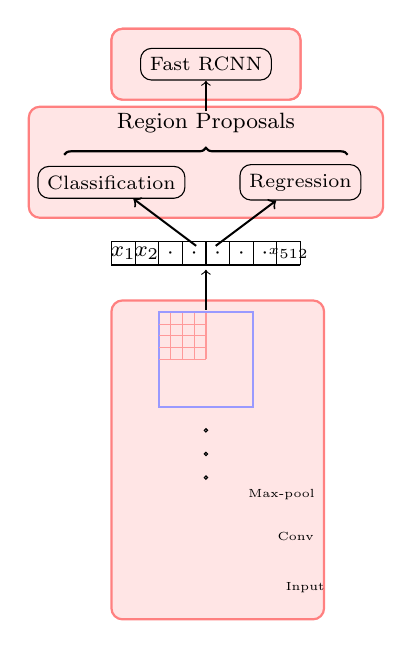
\begin{tikzpicture} [scale=0.30,rotate=90]  
	\onslide<2>{\draw[draw=red!50,fill=red!10,thick,solid,rounded corners] (-2,-6) rectangle (11.5,3); }
	\onslide<3>{\draw[draw=red!50,fill=red!10,thick,solid,rounded corners] (20,-5) rectangle (23,3); }
	\onslide<4>{\draw[draw=red!50,fill=red!10,thick,solid,rounded corners] (15,-8.5) rectangle (19.7,6.5); }
	\onslide<5>{\draw[draw=red!50,fill=red!10,thick,solid,rounded corners] (20,-5) rectangle (23,3); }
	
	\onslide<1->{

		\renewcommand{\forefillColor}{black!50!white}
		\renewcommand{\borderColor}{white}
		\renewcommand{\toprsidefillcolor}{red}

		%% input layer
		\handmadecube{0}{4.5}{2.5}{-1}{0}
		\renewcommand{\toprsidefillcolor}{green}                  
		\handmadecube{0}{4.5}{2.5}{-1+0.2}{0}
		\renewcommand{\toprsidefillcolor}{blue!60!white}          
		\handmadecube{0}{4.5}{2.5}{-1+0.4}{0}
		\node[scale=0.85] at (1-0.6*2.6-0.1,-5.2){\tiny{Input}};
		%     \node [scale=0.7, rotate=45] at (1-0.6*2.6+0.6,0.2) {\tiny{224}};
		%     \node [scale=0.7, rotate=90] at (1-0.6*2.6+0.2,-2) {\tiny{224}};


		% Convolution Layer
		\renewcommand{\forefillColor}{red!50!white}
		\renewcommand{\borderColor}{white}
		\renewcommand{\toprsidefillcolor}{red!50!white!50}

		\pgfmathsetmacro{\seedx}{1}
		\pgfmathsetmacro{\seedy}{0}

		\foreach \xct/\yct in {1,...,2}
		{
			\pgfmathsetmacro{\xcti}{\seedx+\xct*0.1}
			\pgfmathsetmacro{\ycti}{\seedy}
			\handmadecube{0.5}{4.5}{2.5}{\xcti}{\ycti}
		}
		\node[scale=0.85] at (1+0.5,0-4.8){\tiny{Conv}};
		%     \node [scale=0.7, rotate=45] at (1-0.6*2.6+3.2,0.2) {\tiny{224}};
		%     \node [scale=0.7, rotate=90] at (1-0.6*2.6+0.2+2.6,-2) {\tiny{224}};
		
		%     \node[scale=0.7] at (1+0.725,0-4.2){\tiny{64}};
		
		% Pooling Layer
		\renewcommand{\forefillColor}{blue!50!white}
		\renewcommand{\borderColor}{white}
		\renewcommand{\toprsidefillcolor}{blue!50!white!50}
		
		\pgfmathsetmacro{\seedx}{2.5}
		\pgfmathsetmacro{\seedy}{0}

		\foreach \xct/\yct in {1}
		{
			%       \pgfmathsetmacro{\xcti}{\seedx+\xct*0.1}
			%       \pgfmathsetmacro{\ycti}{\seedy}
			
			\pgfmathsetmacro{\xcti}{\seedx+\xct*0.1}
			\pgfmathsetmacro{\ycti}{\seedy}
			\handmadecube{0.5}{3.8}{1.8}{\xcti}{\ycti}
		}
		\node[scale=0.85] at (0.5+2.8,0-4.2){\tiny{Max-pool}};
		%     \node [scale=0.6, rotate=45] at (1+3.7,0.2) {\tiny{112}};
		%     \node [scale=0.6, rotate=90] at (1+3.3,-2+0.5) {\tiny{112}};
		%     \node[scale=0.7] at (1+2.85,0-3.5){\tiny{64}};
		
		\foreach \xct in {1,2,3}
		{
			\filldraw[fill=gray!60](3+\xct,-1) circle(2pt) ;
		}

		\draw [thick,step=1,draw=blue!40!white](7,-3) rectangle (11,1);
		\draw [thin,step=0.5,draw=red!40!white](9,-1) grid (11,1);
		\draw [thin,step=0.5,draw=red!40!white](9,-1) -- (9,1);

		%     \filldraw[fill=green!50!white, draw=black,rounded corners] (13,4) rectangle (14,5);
		\draw [thin,step=1,draw=blue!40!white](7,-3) rectangle (11,1);
		\draw (13,-5) grid[xstep=1,ystep=1] (14,3);     
		\node (x1) at (13.5,2.5) {\footnotesize{$x_1$}};
		\node (x2) at (13.5,1.5) {\footnotesize{$x_2$}};

		\foreach \y in {1,2,...,5}{
			\node (x2) at (13.5,1.5-\y) {\footnotesize{$\cdot$}};
		}

		\node (x2) at (13.5,-4.5) {\tiny{$x_{512}$}};

		\draw[->](11.1,-1)--(12.8,-1);

		\node(A) at (13.5,-1){};
		\node(B)[draw,rounded corners] at (16.5,3){\scriptsize{Classification}};
		\node(C)[draw,rounded corners] at (16.5,-5){\scriptsize{Regression}};
		\node(D)[draw,rounded corners] at (21.5,-1){\scriptsize{Fast RCNN}};
		\path[draw,line width=0.25mm,->] (A) edge (B);
		\path[draw,line width=0.25mm,->] (A) edge (C);
		%\node(D)[draw,rounded corners] at (20.5.5,3){\scriptsize{Classification}};
		\draw[->](19.5,-1)--(20.8,-1);
		\node[font=\fontsize{8}{10}\selectfont] at (19,-1) {Region Proposals};

           
		\draw [
			thick,
			decoration={
				brace,
				raise=0.2cm
			},
			decorate
		] (17,5) -- (17,-7) 
		node [pos=0.1,anchor=north,xshift=-0.5cm,yshift=1.1cm] {};
		

	}
\end{tikzpicture}
		\column{0.5\textwidth}
		\begin{overlayarea}{\textwidth}{\textheight}
			{\bf{\onslide<1->Faster RCNN:Training}}
			\begin{itemize}
				\justifying
				\item<2-> Fine-tune RPN using a pre-trained ImageNet network
				\item<3-> Fine-tune fast RCNN from a pre-trained ImageNet network using bounding boxes from step 1
				\item<4-> Keeping common convolutional layer parameters fixed from step 2,
				fine-tune RPN (post conv5 layers)
				\item <5->Keeping common convolution layer parameters fixed from step 3, fine-tune fc layers of fast RCNN 
			\end{itemize}
		\end{overlayarea}
	\end{columns}
\end{frame}

%%%%%%%%%%%%%%%%%%%%%%%%%%%%%%%%%%%%%%%%%%%%%%%%%%%%%%%%%%%%%%%%%%%%%%%%%%%%%%%%%%%%%%%%%			
			
\begin{frame}
	\begin{block}
		\onslide<1-> Faster RCNN and RPN are the basis of several 1st place entries in the ILSVRC and COCO tracks on :
		\begin{itemize}
			\justifying
			\item<2-> Imagenet detection 
			\item<3-> COCO Segmentation
			\item<4->Imagenet localization
			\item<5-> COCO detection
		\end{itemize}
	\end{block}
\end{frame}

%%%%%%%%%%%%%%%%%%%%%%%%%%%%%%%%%%%%%%%%%%%%%%%%%%%%%%%%%%%%%%%%%%%%%%%%%%%%%%%%%%%%%%%%%			
			
\begin{frame}
	\begin{columns}
		\column{0.5\textwidth}
		\begin{overlayarea}{\textwidth}{\textheight}
			\tikzstyle{input_neuron}=[circle,draw=red!50,fill=red!10,thick,minimum size=4mm]
\tikzstyle{hidden_neuron}=[circle,draw=blue!50,fill=cyan!10,thick,minimum size=4mm]
\tikzstyle{output_neuron}=[circle,draw=green!50,fill=green!10,thick,minimum size=4mm]
\tikzstyle{cpy_neuron}=[circle,draw=red!50,fill=red!50,thick,minimum size=4mm]
\tikzstyle{input}=[circle,draw=black!50,fill=black!20,thick,minimum size=4mm]

\begin{tikzpicture}[scale=0.5, transform shape]
	
	\onslide<1->{
		\node [text width = 30mm] at (2.5,3){Region proposals};
		\node[inner sep=0pt] (A) at (2.5,1.8)
		{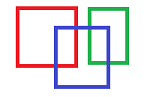
\includegraphics[scale = 0.9]{images/bboxes.png}};

		\node [text width = 34mm] at (6.5,3){Feature extraction};
		\node[inner sep=0pt] (A) at (6.5,2)
		{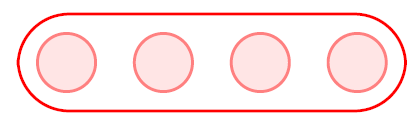
\includegraphics[scale = 0.5]{images/feature.PNG}};
		
		\node [text width = 25mm] at (11.5,3){Classifier};
		\node[inner sep=0pt] (A) at (11.0,2)
		{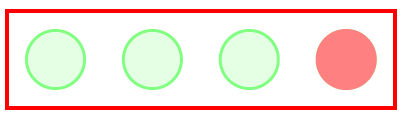
\includegraphics[scale = 0.5]{images/classification.PNG}};
	}
	
	\onslide<1->{
		\node [text width = 25mm] at (0,0){Pre 2012};
		\node[inner sep=0pt] (A) at (2.5,0.2)
		{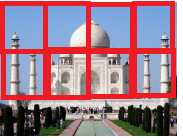
\includegraphics[scale = 0.6]{images/pre_2012.png}};
		\node[inner sep=0pt] (B) at (5.9,0.2)
		{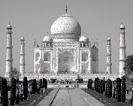
\includegraphics[scale = 0.8]{images/sift.PNG}};
		\node[inner sep=0pt] (C) at (8,0.2)
		{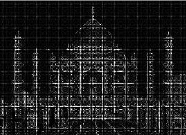
\includegraphics[scale = 0.6]{images/hog.PNG}};
		\node[inner sep=0pt] (D) at (11,0.4)
		{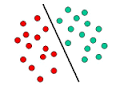
\includegraphics[scale = 0.45]{images/svm.PNG}};
	}
	

	\onslide<1->{
		\node [text width = 25mm] at (0,-1.5){RCNN};
		\node[inner sep=0pt] (A) at (2.5,-1.3)
		{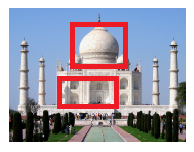
\includegraphics[scale = 0.6]{images/rcnn_bbox.png}};
		\node[inner sep=0pt] (B) at (6.8,-1.4)
		{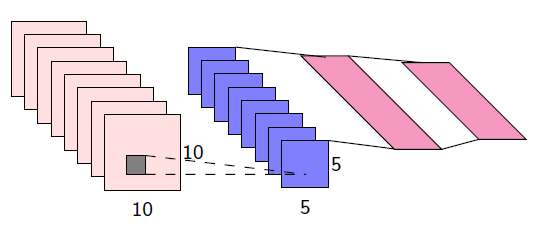
\includegraphics[scale = 0.4]{images/cnn.PNG}};
		\node[inner sep=0pt] (D) at (11,-1.2)
		{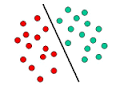
\includegraphics[scale = 0.45]{images/svm.PNG}};
	}
	
	\onslide<1->{
		\node [text width = 25mm] at (0,-3){
		Fast RCNN};
		\node[inner sep=0pt] (A) at (2.5,-2.8)
		{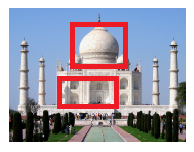
\includegraphics[scale = 0.6]{images/rcnn_bbox.png}};
		\node[inner sep=0pt] (B) at (8.8,-2.9)
		{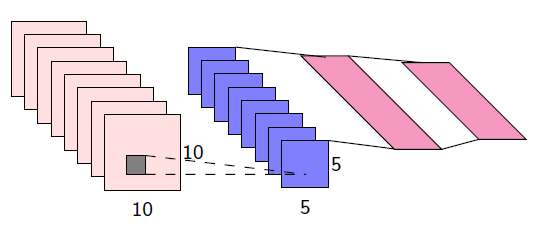
\includegraphics[height=1.5cm,width=6cm]{images/cnn.PNG}};
		%\node[inner sep=0pt] (D) at (11,-2.8)
		%{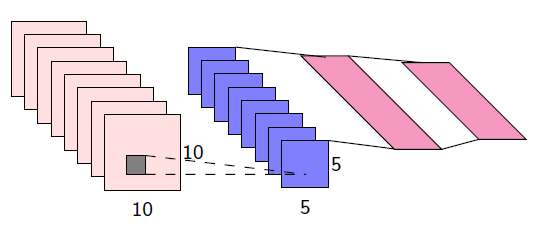
\includegraphics[scale = 0.4]{images/cnn.PNG}};
	}
	
	\onslide<1->{
		\node [text width = 25mm] at (0,-4.8){Faster RCNN};}
	\onslide<2->{\node[inner sep=0pt] (A) at (3,-4.6)
		{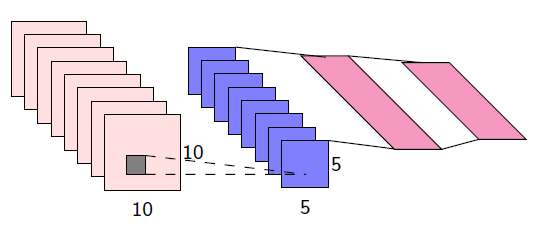
\includegraphics[scale = 0.4]{images/cnn.PNG}};}
	\onslide<3->{\node[inner sep=0pt] (B) at (8.8,-4.6)
		{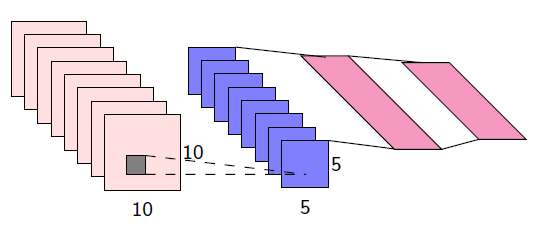
\includegraphics[height=1.5cm,width=6cm]{images/cnn.PNG}};}
	%\onslide<4->{\node[inner sep=0pt] (D) at (11,-4.5)
	%	{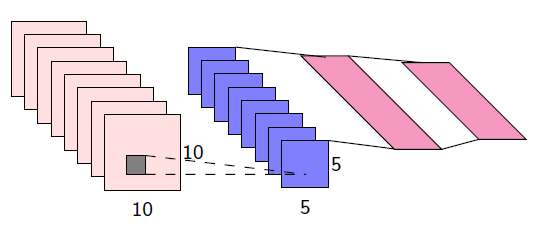
\includegraphics[scale = 0.4]{images/cnn.PNG}};}
\end{tikzpicture}
			
		\end{overlayarea}
		\column{0.5\textwidth}
		\begin{overlayarea}{\textwidth}{\textheight}
			\begin{itemize}
				\item<2-> \textbf{Region Proposals:} CNN
				\item<3-> \textbf{Feature Extraction:} CNN
				\item<4-> \textbf{Classifier:} CNN
			\end{itemize}
		\end{overlayarea}
	\end{columns}
\end{frame}

%%%%%%%%%%%%%%%%%%%%%%%%%%%%%%%%%%%%%%%%%%%%%%%%%%%%%%%%%%%%%%%%%%%%%%%%%%%%%%%%%%%%%%%%%

\begin{frame}
	\begin{overlayarea}{\textwidth}{\textheight}
		\begin{figure}
			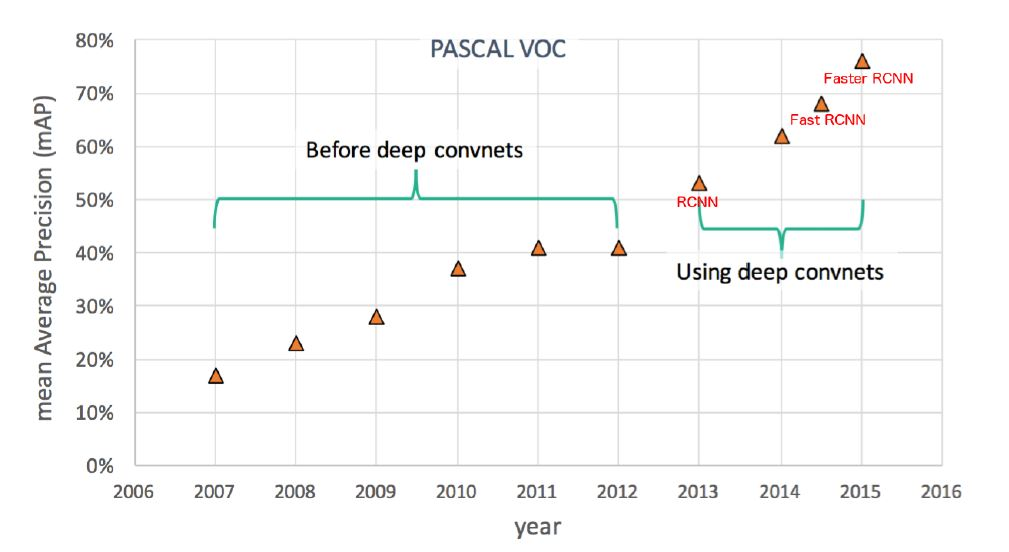
\includegraphics[scale =0.65]{images/object.JPG}
			\caption{Object Detection Performance } \hspace{10cm} Source: Ross Girshick
		\end{figure}
	\end{overlayarea}
\end{frame}
